\documentclass[a4paper]{article}

\usepackage[english]{babel}
\usepackage{amsmath}
\usepackage{float}
\usepackage{amssymb}
\usepackage{dsfont}
\usepackage{graphicx}
\usepackage{listings}
\usepackage[hyphens]{url}
\usepackage{titling}
\usepackage{varwidth}
\usepackage{hyperref}
\usepackage{color} %red, green, blue, yellow, cyan, magenta, black, white
\definecolor{mygreen}{RGB}{28,172,0} % color values Red, Green, Blue
\definecolor{mylilas}{RGB}{170,55,241}



\usepackage{geometry}
 \geometry{
 a4paper,
 total={165mm,257mm},
 left=20mm,
 top=20mm,
 }

\title{Web Security\\Assignment 2}
\author{
  Christoph Schmidl\\ s4226887\\ Data Science\\      \texttt{c.schmidl@student.ru.nl}
}
\date{\today}

\begin{document}
\maketitle

\begin{enumerate}

\item Do the following two lessons in WebGoat (you do not have to submit any notes regarding these exercises to blackboard):

	\begin{itemize}
		\item Session Management Flaws - Hijack a Session
		
		\begin{figure}[H]
	    \centering
  	    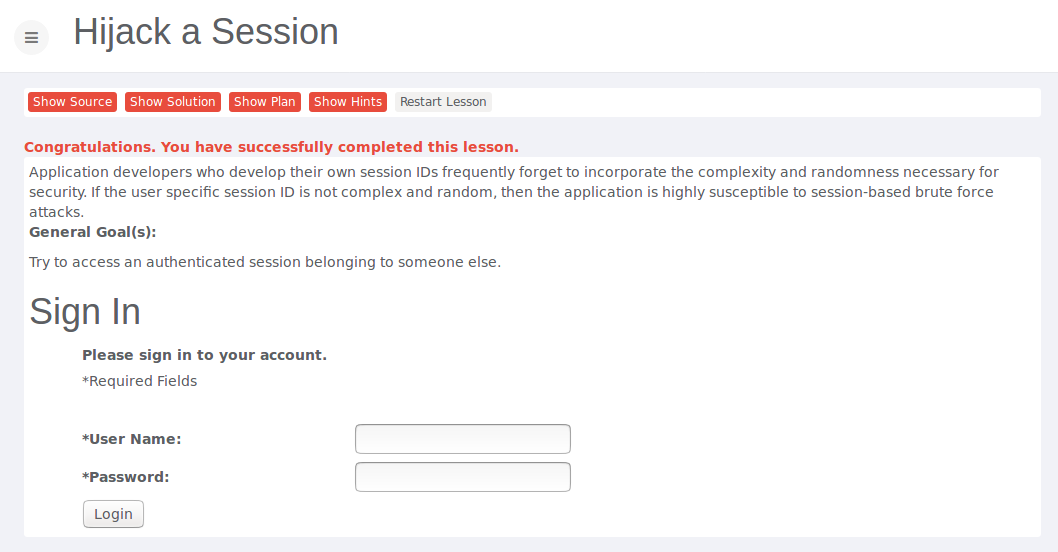
\includegraphics[width=0.8\textwidth]{img/hijack_a_session_screen.PNG}
	    \end{figure}	
	    
	    Session hijacking, sometimes also known as cookie hijacking is the exploitation of a valid computer session - sometimes also called a session key - to gain unauthorized access to information or services in a computer system. In particular, it is used to refer to the theft of a magic cookie used to authenticate a user to a remote server. In this particular lesson the value of the cookie named "WEAKID" can be bruteforced by using a tool like JHijack. To find a value to start with you can use the SessionID Analysis Tab of WebScarab. You do not know the identity of the user's session you are going to hijack beforehand.\\
	    
		\item Session Management Flaws - Session Fixation
		
		\begin{figure}[H]
	    \centering
  	    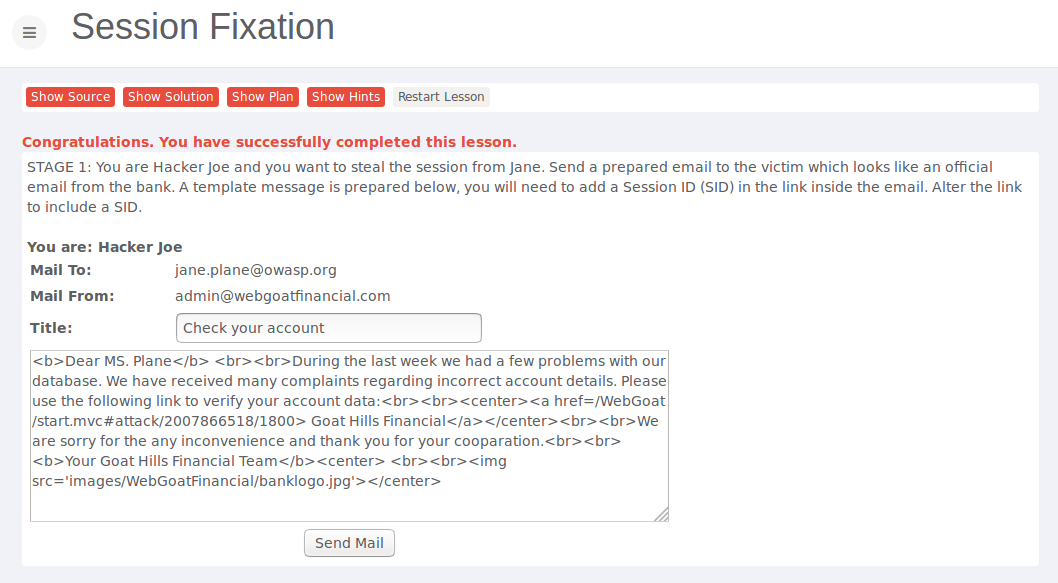
\includegraphics[width=0.8\textwidth]{img/session_fixation_screen.PNG}
	    \end{figure}	
	\end{itemize}

Session fixation attacks attempt to exploit the vulnerability of a system that allows one person to fixate (find or set) another person's session identifier. Most session fixation attacks are web based, and most rely on session identifiers being accepted from URLs (query string) or POST data. A misconception is that if a server only accepts server-generated session identifiers, it is safe from fixation. This is false.\\


\item Inspect 5 websites for which you got login credentials
	\begin{itemize}
		\item Do these website use HSTS (HTTP Strict Transport Security)?
		\item Does the session ID cookie of these websites use \textit{Secure} and/or \textit{HttpOnly}?
	\end{itemize}

Make a table of these websites and their support for HSTS, the name of the cookie and the usage of \textit{Secure} and \textit{HttpOnly} for that cookie.\\
\textbf{Solution:}\\

\begin{table}[h!]
\centering
\label{my-label}
\begin{tabular}{|c|l|c|c|l|}
\hline
\textbf{Website} & \textbf{HSTS} & \textbf{Cookie Name}  & \textbf{Secure} & \textbf{HttpOnly} \\ \hline
facebook.com  & yes &   multiple cookies (c\_user, xs, sb)  & yes, yes, yes                      & no, yes, yes \\ \hline
mail.ru.nl   & no &  cadata                     &   yes                    & yes  \\ \hline
linkedin.com  & no & li\_at                      &    yes                   & yes  \\ \hline
github.com  & yes &   	\_gh\_sess                    &  yes                     & yes  \\ \hline
gmx.net & yes & 905a7a5991a00898953878290a55d118 & yes & yes \\ \hline
\end{tabular}
\caption{Website Information}
\end{table}


\end{enumerate}

\end{document}